
\documentclass[11pt,twoside]{article}

\usepackage[utf8]{inputenc}
\usepackage{graphicx}
\usepackage{amsmath}
\usepackage{amssymb}
\usepackage{url}
\usepackage{graphics}
\usepackage{wasysym}
\usepackage{enumitem}
\usepackage[english,portuges]{babel}
\usepackage{color}
\usepackage[usenames,dvipsnames]{xcolor}



\begin{document}

%*********************************************************************** TITULO

\section*{Esquema de interpolação alternativo para a reso\-lução numérica de
problemas de difusão com convecção usando o método dos volumes finitos}

\vspace{10pt}


%************************************************************************* AUTORES
Luís J.M. Amoreira$^{1}$%, Nome Sobrenome$^{1,2}$, Nome Sobrenome$^{1,2}$

\vspace{10pt}


%************************************************************************** MORADA

{
\center

    \footnotesize

$^{1}$ Departamento de Física, Universidade da Beira Interior, Covilhã,
Portugal\\
E-mail: amoreira@ubi.pt
%
%\vspace{3pt}
%
%$^{2}$ Endereço 2, Portugal \\
%Email:  email2@email.pt
%
%\vspace{3pt}
%
%$^{3}$ Endereço 1, Portugal

}

\vspace{25pt}

%%%%%%%%%%%%%%%%%%%%%%%%%%%%%%%%%%%%%%%%%% RESUMO


{\setlength{\parindent}{30pt}%

\small%
\section*{Resumo}
\smallskip
%%%%%%%%%%%%%%%%
%Corpo do resumo (aprox. 200 palavras)
Neste trabalho é proposto um esquema de discretização alternativo para a
resolução de problemas de difusão com convecção baseado no esquema de diferenças
centrais mas com coeficientes de interpolação que dependem da velocidade do fluxo
convectivo.

É feita uma análise comparativa do esquema proposto com esquemas tradicionais
(diferenças centrais, \emph{upwind}, híbrido) em termos da estabilidade, da
exatidão e da taxa de convergência. O problema usado para a comparação é o da
difusão estacionária unidimensional sem fontes, num fluido incompressível em
escoamento com velocidade constante, para o qual existem soluções analíticas.

Verifica-se que o esquema proposto é estável mesmo em problemas com convecção
intensa e que produz, em geral, resultados mais aproximados da solução analítica
dos que os obtidos com os restantes esquemas considerados. Como o esquema de
diferenças centrais, o esquema proposto é de segunda ordem em malhas homogéneas
centradas.

\vspace{15pt}





%%%%%%%%%%%%%%%%%%%%%%%%%%%%%%%%%%%%%%%%%%%    SECTIONS  %%%%%
\section{Introdução}
%Corpo de texto regular, com referencias do estilo [1] e [2, 3]. as referências
%devem ser introduzidas manualmente. O estilo das referências é definido pelos
%editores.
Na resolução numérica de equações de conservação como as que normalmente surgem
em problemas de dinâmica de fluidos usando o método dos volumes finitos,
define-se uma partição do domínio de integração com um conjunto de subdomínios
finitos chamados \emph{volumes de controle} (VC) e integram-se as equações
diferenciais a resolver em cada um desses subdomínios. Resulta deste
procedimento um sistema de equações algébricas que relacionam os valores dos
fluxos característicos do problema através das fronteiras dos vários VC. A
resolução deste sistema de equações algébricas produz os valores aproximados dos
campos a determinar nos pontos característicos de cada VC (frequentemente,
tomam-se os seus centros geométricos).  Este procedimento passa por estabelecer
relações entre os fluxos nas faces dos VC e os valores dos campos nos pontos da
malha de discretização. Na prática, essas relações obtêm-se a partir de
fórmulas de cálculo dos valores dos campos (para fluxos do tipo convectivo, proporcionais aos campos) e dos seus gradientes (para os de tipo difusivo, proporcionais aos gradientes dos campos) nas faces dos VC a partir dos valores dos campos no centros dos VC. Essas fórmulas definem o chamado \emph{esquema de discretização} usado.

Os esquemas de discretização mais simples considerados no estudo de problemas de
difusão acompanhada de convecção (os abordados no presente trabalho) são (1) o
\emph{esquema de diferenças centrais} (CDS) [REFS], em que se estimam os valores
dos campos nas faces por interpolação linear e os dos seus gradientes com a
fórmula de derivação central; (2) o \emph{esquema de diferenças upwind} (UWS)
[REFS], que difere do CDS apenas na expressão dos valores dos campos nas faces
dos  VC, tomando-se simplesmente iguais aos seus valores no VC ``a montante''
no escoamento; (3) o \emph{esquema de híbrido} (HDS) [REFS] em que se adota o
CDS em problemas de escoamento lento e o UWS (desprezando-se ainda os termos
difusivos) quando o escoamento é rápido.

O primeiro destes esquemas (CDS) apresenta problemas de estabilidade em
situações caracterizadas por escoamentos rápidos, em que o transporte convectivo
domina o difusivo, que são resolvidos no segundo (UWS), mas à custa de soluções
afetadas de maior erro, especialmente quando o escoamento do meio material é
lento, ou seja, quando o  difusivo é o dominante[REFS]. O esquema híbrido é
satisfatório principalmente nos casos extremos (escoamento muito lento ou muito
rápido) mas menos em regimes próximos da situação discriminante. Além disso,
pode gerar soluções com descontinuidades temporais em problemas não
estacionários, quando as condições do escoamento se alteram de modo a ser
trocado o esquema (CDS ou UWS) adotado.

Neste trabalho sugere-se um esquema simples alternativo (designado como
\emph{esquema de ajuste contínuo,} CAS), que resultados
preliminares indicam que poderá apresentar vantagens face aos três referidos
acima. O esquema  proposto é semelhante ao esquema de diferenças centrais, mas os
coeficientes de interpolação usados na estimativa dos valores dos campos nas
faces dos VC dependem, de forma contínua, da importância relativa dos
transportes difusivo e convectivo.

\subsection{Difusão com convecção estacionária unidimensional}
Os quatro esquemas considerados neste trabalho são comparados por aplicação na
resolução de um problema particularmente simples, o da difusão estacionária e
unidimensional de uma propriedade extensiva conservada num fluido incompressível
com densidade de massa $\rho$ em escoamento com velocidade de módulo $v$, na
ausência de fontes. Seja $\phi$ o valor da propriedade por unidade de massa
($\rho\phi$ é, assim a sua densidade espacial) e $\Gamma$ o coeficiente de
difusão relevante (considerado uniforme). A equação que descreve a conservação
desta propriedade ao nível local é[REFS]
\begin{equation}
    \frac{d^2\phi}{dx^2}=\mu\frac{d\phi}{dx}, \qquad \mu=\frac{\rho v}{\Gamma}.
    \label{eq:10}
\end{equation}
A solução analítica desta equação no intervalo $0<x<L$ que satisfaz as condições
fronteira $\phi(0)=\phi_0$ e $\phi(L)=\phi_L$ é
\begin{equation}
    \phi(x) = \phi_0 + (\phi_L-\phi_0)\frac{e^{\mu x}-1}{e^{\mu L}-1}.\label{eq:15}
\end{equation}

Faça-se agora uma abordagem numérica a este problema usando o método dos
volumes finitos. Considera-se uma partição do intervalo de integração em
subintervalos, como se ilustra na Figura~\ref{fig:10}.
%%%%%%%%%%%%%%%%%%%%%%%%%%% FIGURA
\begin{figure}[!h]
\centering
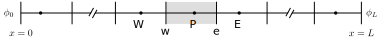
\includegraphics[scale=0.95]{figs/f10.png}
\caption{Partição do domínio de integração num conjunto de volumes de
controle.\label{fig:10}}
\end{figure}
A integração da eq.~\eqref{eq:10} no volume do VC destacado na figura resulta em
\begin{equation}
    \left(\frac{d\phi}{dx}\right)_e- \left(\frac{d\phi}{dx}\right)_w =
    \mu(\phi_e-\phi_w).
\end{equation}
Aplicando a fórmula da derivada central no cálculo das derivadas no lado
esquerdo (e recorde-se que esse procedimento é seguido nos vários esquemas
discutidos), obtém-se
\begin{equation}
    \phi_E-2\phi_P+\phi_W=P(\phi_e-\phi_w),\label{eq:20}
\end{equation}
onde o parâmetro adimensional $P=\mu\delta x=\rho v\delta x/\Gamma$, chamado
\emph{número de Peclet,} é usado para indicar a importância relativa dos
transportes convectivos e difusivos. Quanto maior o seu módulo, maior a
importância da convecção; ao contrário, $|P|<<1$ sinaliza situações em que a
difusão é dominante.

\section{O esquema de ajuste contínuo (CAS)}
O CAS distingue-se do esquema de diferenças centrais pela expressão adotada para
os valores dos campos nas faces dos VC [$\phi_e$ e $\phi_w$, na
eq.~\eqref{eq:20}]. Concretamente, e considerando para simplificar uma malha
homogénea e centrada (em que as faces dos VC se encontram a iguais distâncias
dos dois pontos da malha vizinhos), aplicam-se as igualdades
\begin{align}
    \phi_e &= f(P)\phi_P + [1-f(P)]\phi_E&
    \phi_w &= f(P)\phi_W + [1-f(P)]\phi_P,
\end{align}
onde os coeficientes de interpolação $f$ e $(1-f)$ são função do valor do número
de Peclet, dados por
\begin{equation}
    f(P)=\frac12\left(1+\frac{P}{\xi+|P|}\right),\qquad\xi>0.
\end{equation}
O parâmetro real positivo $\xi$ pode ser escolhido da forma considerada mais
conveniente em cada caso. Neste trabalho, em que as soluções analíticas estão
disponíveis, $\xi$ é fixado de modo a minimizar o erro das soluções numéricas
numa gama alargada de regimes de escoamento, como se discute na próxima secção.
Na Figura~\ref{fig:20} está representado o gráfico desta função.
%%%%%%%%%%%%%%%%%%%%%%%%%%% FIGURA
\begin{figure}[!h]
\centering
\includegraphics[scale=0.95]{figs/f20.pdf}
\caption{Coeficiente de interpolação $f$ como função do número de Peclet.
\label{fig:20}}
\end{figure}
Com os coeficientes de interpolação assim definidos, dá-se uma maior importância 
o valor do campo no ponto de malha situado a montante, e esse incremento de
importância é tanto maior quanto maior (em módulo) for o número de Peclet, ou
seja, a velocidade de escoamento.


\section{Resultados da comparação}
Uma vez estabelecido o esquema de discretização, a resolução numérica da
eq.~\eqref{eq:10} segue linhas bem estabelecidas (ver, por exemplo, [REFS]). Usaram-se os 
quatro esquemas referidos para obter soluções considerando um fluido com densidade $\rho=1,0$\,kg/m$^3$ e coeficiente de difusão $\Gamma=0,1$\,kg/m/s, movendo-se com velocidade $v=2,5$\,m/s no sentido positivo ($\mu=25$\,m$^{-1}$), numa malha de cinco pontos equidistantes. Na aplicação do esquema de ajuste contínuo, foi inicialmente fixado o valor do parâmetro $\xi$ da função de interpolação. Escolheu-se a média aritmética dos
valores que minimizam o erro dos resultados obtidos para cinquenta valores da
velocidade de escoamento definidos no intervalo [0,5], correspondendo a números
de Peclet na gama $0<P<10$. O valor obtido foi $\xi\simeq7,293$.

Na Figura~\ref{fig:30} à esquerda mostram-se os valores das soluções numéricas obtidas com os quatro esquemas nos pontos da malha usada, juntamente com a representação gráfica da solução analítica da eq.~\eqref{eq:15}.
%%%%%%%%%%%%%%%%%%%%%%%%%%% FIGURA
\begin{figure}[!h]
\centering
\includegraphics[scale=0.9]{figs/f30.pdf}\hfill
\includegraphics[scale=0.9]{figs/f40.pdf}
\caption{Soluções obtidas com os quatro esquemas num problema com $\mu=25\,\text{m}^{-1}$, usando uma malha de cinco pontos (à esquerda) e comparação do valor do erro das soluções para diferentes valores do número de Peclet (à direita).
%a gama indicada corresponde a valores de $mu$ no intervalo $0<\mu<40\,\text{m}^{-1}$.
\label{fig:30}}
\end{figure}
São patentes na figura os problemas de estabilidade do esquema CDS. É também
claro que o esquema CAS é o que produz resultados mais próximos da solução
analítica, sendo essa exatidão notável dada a malha grosseira usada nesta
análise.

Esta superior exatidão do esquema de ajuste contínuo verifica-se para diferentes
velocidades de escoamento. Para o verificar, foi comparado o erro das diferentes
soluções numéricas para diferentes valores da velocidade do escoamento. Como medida do
erro usou-se a norma-$l_2$ da diferença entre as soluções numérica e analítica,
definida como
\begin{equation}
    \epsilon = \sqrt{\frac{1}{N}\sum_{i=1}^N(\phi^*_i-\phi(x_i))^2},
\end{equation}
onde $N$ é o número de pontos na malha de discretização, e $\phi^*_i$ e
$\phi(x_i)$ são, respetivamente, as soluções numérica e analítica para o
$i$-ésimo ponto. Naturalmente, o valor do parâmetro $\xi$ do esquema de ajuste
contínuo foi mantido sempre com o valor já indicado. Os resultados obtidos estão apresentados na Figura~\ref{fig:30} à direita, como função do número de Peclet.
Constata-se que o CAS apresenta de facto erros significativamente menores que os
restantes esquemas e revela uma muito menor sensibilidade ao regime de
escoamento. A figura revela também uma descontinuidade gerada pelo esquema
híbrido do tipo das referidas na introdução: para $P=2$, o valor do erro cai
bruscamente (indicando uma alteração igualmente descontínua da solução encontrada), quando o HDS substitui o procedimento adotado em escoamentos lentos
(CDS) pelo adotado em escoamentos rápidos (UWS sem difusão).

Para valores do número de Peclet próximos de zero, o esquema híbrido \emph{é} o esquema de diferenças centrais e de ajuste contínuo são equivalentes, e o esquema de ajuste contínuo vai-se tornando cada vez mais semelhante a esses dois à medida que $P\rightarrow0$. Por isso, o HDS e o CAS apresentam ambos taxas de convergência semelhantes à do CDS, que, em malhas homogéneas e centradas, é um esquema de segunda ordem.  Esta propriedade é ilustrada na Figura~\ref{fig:50}: os erros dos três esquemas referidos dispõem-se ao longo de linhas paralelas que, na escala logarítmica do gráfico, têm declive $m\simeq2$. Já o UWS, que desvaloriza de forma grosseira os fluxos difusivos nas faces dos VC, apresenta uma taxa de convergência muito menor ($m\simeq0,77$).
\begin{figure}[!h]
\centering
\includegraphics[scale=0.9]{figs/f50.pdf}
\caption{Taxas de convergência dos quatro esquemas comparados. \label{fig:50}}
\end{figure}

%%%%%%%%%%%%%%%%%%%%%%%%%%% TABELA
%\begin{table}[!h]
%\caption{Legenda da tabela.}
%
%\end{table}



%%%%%%%%%%%%%%%%%%%%%%%%%%% FIGURA
%\begin{figure}[!h]
%\centering
%\includegraphics[scale=0.95]{fig_1.pdf}
%\caption{Legenda da figura.}
%\end{figure}








%%%%%%%%%%%%%%%%%%%%%%%%%%%%%%%%%%%%%%%%%%%    SECTION  %%%%%
\section{Conclusões}

\begin{itemize}

\item O esquema proposto neste trabalho revelou-se superior, em termos de
    estabilidade e de exatidão, aos esquemas simples tradicionalmente
    considerados.
\item O CAS é mais robusto que os esquemas tradicionais, no sentido em que o
    erro das suas soluções é quase independente das condições do escoamento.
\item O CAS apresenta ainda taxas de convergência significativamente superiores
    aos dos restantes métodos estudados.


\end{itemize}




%%%%%%%%%%%%%%%%%%%%%%%%%%%%%%%%%%%
%%
%%                 AKNOWLEDGMENTS & BIBLIOGRAPHY
%%
%%%%%%%%%%%%%%%%%%%%%%%%%%%%%%%%%%%

{\footnotesize%


%%%%%%%%%%%%%%%%%%%%%%%%%%%%%%%%%%%%%%%%%%%    AGRADECIMENTOS  %%%%%
%\section*{Agradecimentos}
% Text







%%%%%%%%%%%%%%%%%%%%%%%%%%%%%%%%%%%%%%%%%%%    REFERÊNCIAS  %%%%%
\section*{Referências}
\vspace{5pt}

\begin{enumerate}[label={[\arabic*]}]

\item	Laugksch R., Scientific Literacy: A Conceptual Overview Science Education, 84, 71-94, 2000.

\item	Driver, R., Young people's images of science, Open University Press (Buckingham and Bristol, PA) 1996.

\item	Lopes J.B., Pinto J., Silva, A. Situação formativa: um instrumento de gestão do currículo capaz de
promover literacia científica. Enseñanza de las Ciencias, Número Extra VIII Congreso Internacional sobre
Investigación en Didáctica de las Ciencias, Barcelona, pp. 1624-1629 2009.



\end{enumerate}

}


\end{document}
